\chapter{مروری بر کارهای پیشین}

\section{مقدمه}
در این فصل، به مرور کارهای گذشته می‌پردازیم.
ابتدا صورت مسئله مقالات مختلف را بررسی می‌نماییم که
 به ترتیب شامل مقالاتی هستند که از برش شبکه استفاده کرده اند.
برش شبکه در سه بخش رادیویی، بخش هسته و هردو بخش هسته و رادیویی صورت می‌گیرد.
سپس در زمینه ی سیر عبور از شبکه های دسترسی رادیویی ابری به شبکه های دسترسی رادیویی باز مطالعه نموده و بعد از آن درباره ی جاگیری VNF ها صحبت می‌کنیم.
سپس در مورد روش حل مسئله صحبت می‌کنیم که شامل مسائل کوله پشتی و بسته بندی جعبه می‌باشد و در نهایت در مورد روشهای یادگیری تقویتی صحبت می‌کنیم.
\section{مسائل حل شده}
در این بخش به مطالعه ی مسائل پیش رو می‌پردازیم. ‌‌‌
\subsection{برش شبکه}
برش شبکه یک شبکه منطقی انتها به انتهای مستقل است که بر روی یک زیرساخت فیزیکی مشترک کار ‌ و قادر به ارائه خدمات می‌باشد.
در این بخش برش شبکه در بخش رادیویی و هسته و هردو را بررسی می‌کنیم.
%\subsection{برش شبکه در شبکه های دسترسی رادیویی }
برش RAN یکی از کلیدهای اصلی برای انعطاف پذیری سفارشات و مدیریت مجازی سازی ایستگاه پایه می‌باشد تا بتواند منابع رادیویی را در میان سرویس های مختلف تقسیم کرده و منجر به سازگاری اپراتورها و برطرف کردن نیاز سرویس ها گردد.
%در ادامه مروری بر این مدل مقالات می‌نماییم.
%\subsubsection{  برش شبکه در شبکه های دسترسی رادیویی ابری و متجانس و مهی}

شبکه های دسترسی رادیویی ابر (C-RAN) به عنوان یک چارچوب امیدوار کننده برای سیستم های ارتباط بی سیم نسل پنجم ظاهر شده‌اند.
از آنجا که آنها میتوانند پیچیدگی رمزگشایی، مصرف انرژی و دخالت های ناشی از افزایش تراکم تلفن همراه را کاهش دهند\cite{cranInt}.
در ادامه در مورد برش شبکه در بخش رادیویی شبکه های دسترسی رادیویی ابری صحبت می‌کنیم.

در مقاله‌ی \cite{lee2018dynamic}
برش شبکه به صورت دینامیکی در بخش رادیویی مورد بررسی قرار گرفته شده‌است.
برش شبکه در اینجا به عنوان فرآیند تخصیص منابع شبکه به کاربران انجام ‌
چارچوب طرح برش شبکه شامل یک سطح بالاتر، که مدیریت کنترل پذیرش کاربران، ارتباط کاربر که شامل تخصیص واحد رادیویی (RRH) برای بیشینه سازی نرخ کاربران و تخصیص ظرفیت منابع باند پایه (‌BBU) و یک سطح پایین تر، که تخصیص توان و بلوک منابع فیزیکی (PRB) در میان کاربران می‌باشد.
در این مدل فرض می‌کنیم که هر سرویس دارای شبکه اصلی خود (یا قطعه اصلی شبکه) است که به H-CRAN متصل می‌شود.
سلول بزرگ RRH (M-RRH) و سلولهای کوچک RRHs (S-RRHs) به ترتیب از طریق پیوندهای پشتی و fronthaul به یک استخر ابر
BBU  متصل میشوند.
همچنین ، تقسیم C/U در مدل سیستم فرض می‌شود، که به موجب آن صفحات کنترل و داده از هم جدا میشوند به گونه ای که صفحات کنترل توسط M-RRH در شبکه مدیریت می‌شود.
\begin{figure}%[H]
  \centering
    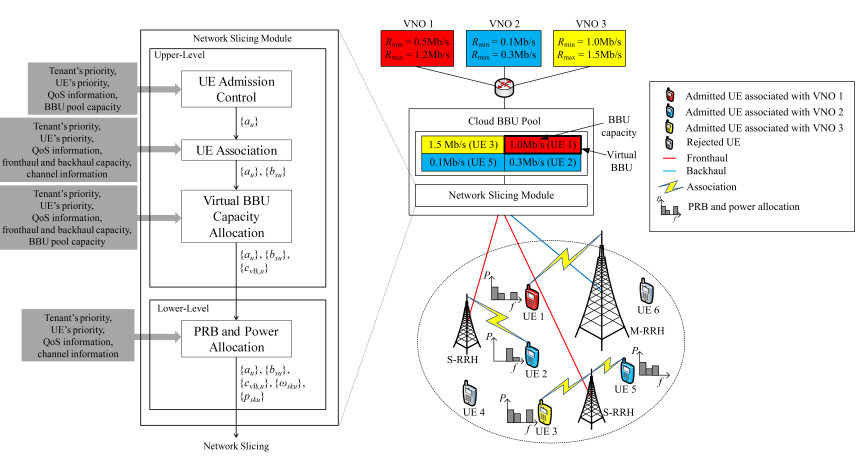
\includegraphics[scale = 0.7]{./fig/dynamicNS}
  \caption{روند برش شبکه\ \cite{lee2018dynamic}}
  \label{fig:dns}
\end{figure}
%برای حل این مسئله، میبایست مسئله را به بخش های کوچکتر تقسیم کرده و حل نماییم.
همانطور که در شکل \eqref{fig:dns} 
مشخص شده‌است ابتدا پذیرش کاربر مورد توجه قرار می‌گیرد و سپس کاربر به RRH متصل می‌شود و پس از آن ظرفیت BBU به آن تخصیص می‌دهد که تا این بخش از کار در سطح بالا قرار داریم.
در سطح بالا، یک مسئله کنترل پذیرش با برنامه نویسی پویا می‌باشد که در آن پیچیدگی را میتوان تنظیم کرد.
این مسئله از جنس مسئله ی
کوله پشتی \LTRfootnote{Knapsack}
باینری
 می‌باشد که با الگوریتم دینامیکی جواب بهینه ی آن بدست میآید.
همچنین مسئله ی ارتباط کاربر نیز یک مسئله ی کوله پشتی باینری است که با استفاده از یک الگوریتم حریص با پیچیدگی کم بهینه و حل می‌شود.
 مسئله ی تخصیص ظرفیت BBU نیز فرموله شده و با برنامه ریزی خطی حل می‌شود.
 حال وارد الگوریتم سطح پایین تر میشویم که تخصیص توان و منبع فیزیکی می‌باشد.
برای مساله ی سطح پایین تر، مشکل تخصیص منابع به عنوان یک مشکل برنامه نویسی mixed-integer غیر محدب است که با استفاده از روش دوگانه لاگرانژ حل می‌شود.

در مقاله‌ی 
\cite{larsen2018fronthaul,costanzo2018network}
برش شبکه در شبکه های دسترسی رادیویی ابری مورد توجه قرار گرفته است. 
در بخش fronthaul مشکلاتی از قبیل پیچیدگی شبکه و محدودیت نرخ وجود دارد که در برش شبکه، منجر به بهبود آن می‌شود.
علاوه بر این ، C-RAN میتواند مجازی سازی مجموعه ای از توابع RAN را امکان پذیر کرده و راه را برای اصطلاحاً RAN مجازی باز کند. با این کار میتوان چندین شبکه مجازی یا برش ایجاد کرد.
 مقاله‌ی
\cite{larsen2018fronthaul}
نشان داده است که استفاده از برش شبکه و برخورداری از سوییچ بسته در fronthaul
مزایای زیادی را به همراه خواهد داشت که از جمله برخورداری از تقسیمات عملکردی مختلف خواهد بود. همچنین از معایب این کار تاخیر نسبتا اندکی می‌باشد.

در مقاله‌ی 
\cite{fran}
برش شبکه در بخش رادیویی برای ساختار مه \LTRfootnote{Fog Radio Access Network}
 یا F-RAN
  در نظر گرفته شده‌است که در آن دو نمونه برش شبکه برای هات اسپات و سناریوهای وسیله نقلیه با زیرساخت مربوط تنظیم می‌شود. به طور خاص ، چارچوب برای برش RAN به عنوان یک مشکل بهینه سازی مشترک برای مقابله با ذخیره کردن و انتخاب حالت است.
  با توجه به خواسته های کاربران مختلف و منابع محدود، پیچیدگی مسئله بهینه سازی اصلی بسیار زیاد است و همین امر باعث می‌شود که رویکردهای بهینه سازی سنتی به طور مستقیم سخت باشد.
 برای مقابله با این معضل ، یک الگوریتم یادگیری تقویت عمیق ارائه شده‌است ، که ایده اصلی آن این است که سرور ابر تصمیمات صحیحی را در زمینه ذخیره محتوا و انتخاب حالت برای به حداکثر رساندن عملکرد پاداش در وضعیت کانال پویا و وضعیت حافظه نهان ارائه می‌دهد.
%\subsubsection{برش شبکه در شبکه های دسترسی رادیویی }

در مقاله‌ی 
\cite{ranSlice, ranSlice1}
اجرای مفهوم برش در سطح RAN توسط اپراتور شبکه تلفن همراه (MNO) برای پاسخگویی به نیازها می‌باشد. همچنین مساله ی تخصیص منابع (در اینجا پهنای باند) مورد توجه قرار گرفته شد.
چالش های پیش رو برش RAN نیز مورد بررسی قرار گرفته است که یکی از چالش ها
شامل طراحی و مدیریت چندین برش در زیرساخت مشترک به روشی کارآمد و در عین حال ضمانت SLA توافق شده برای هر یک از آنها است.
این چالش ما را نیازمند مفهوم ایزولاسیون برش می‌کند.

در مقاله‌ی 
\cite{ranslice2}
برش در بخش RAN مورد توجه قرار گرفته است.
همچنین
در این مقاله‌یک برنامه تخصیص منابع پویا، با هدف به طور مشترک بهینه سازی مصرف برق و تخصیص پهنای باند در حالی که رضایت از تأخیر مربوطه برای ورود ترافیک پراکنده uRLLC و کیفیت خدمات eMBB را تا حد ممکن ارائه می‌دهد، پیشنهاد می‌کند.
طرح پیشنهادی براساس کنترل بهینه توان برای تخصیص منابع آگاه از تأخیر است.
در نتیجه در این سیستم هدف مینیمم کردن توان با شروط برآورده شدن شروط پهنای باند و  تاخیر که با شرط صف پردازش نشان داده، می‌باشد.
%\subsection{برش شبکه در بخش هسته  }

در مقاله‌ی 
\cite{onet}
اجرای عملی برش شبکه پیشنهاد شده‌است.
در مدل پیشنهادی، نویسندگان فرض میکنند که در هر شکاف زمانی مشخص، کاربران فقط میتوانند یک برش شبکه واحد را درخواست کنند.
در اینجا تابع هدفی بر اساس نسبت میزان منابع اختصاص داده شده به کاربرن در هر زمان t به ظرفیت کل منابع مشخص شده‌است و هدف بیشینه سازی آن  می‌باشد.  
مدل پیشنهادی بر اساس مسئله \lr{multi armed bandit} ساخته شده‌است و نویسندگان سه نوع  آن را برای حل جنبه های مختلف تخصیص برش شبکه معرفی کرده اند.
آنها با استفاده از MATLAB مدل بهینه سازی را شبیه سازی کرده و نتایج را با یک الگوریتم حریص مقایسه کردند. آنها همچنین اثبات مفهوم برش شبکه را ارائه دادند.

برش شبکه یکی از فناوری های کلیدی است که به شبکه های 5G اجازه می‌دهد منابع اختصاصی به صنایع مختلف (خدمات) ارائه دهند.
در مقاله‌ی
\cite{li2019latency}
نویسندگان یک روش تخصیص منابع (تأخیر بهینه) برای برشهای شبکه حمل و نقل 5G برای پشتیبانی از خدمات URLLC ارائه داده اند.
آنها ویژگی های منبع شبکه و ویژگی های توپولوژی تخصیص منابع در تقسیم شبکه را معرفی کردند.

در 
\citep{vnf1,coreSlice}
ایزوله کردن برش شبکه ی هسته 
مورد توجه قرار گرفته است.
\citep{vnf1}
برای کاهش تأثیر حملات DDoS در احراز هویت برش ، از ایزوله کردن برش شبکه ی هسته استفاده شده و حل آن با ترکیبی از شبیه سازی و یک آزمایش عملی ارزیابی شده‌است.
نویسندگان
\citep{coreSlice}
دو چالش مهم برش شبکه در بخش هسته مورد توجه قرار داده اند که شامل ایزوله کردن برش شبکه و تضمین میزان تاخیر انتها به انتها می‌باشد.
در این مقاله، مساله ی بهینه سازی به صورت 
\lr{mixed integer linear programming}
 می‌باشد که
 تابع هدف درخواست های برش ورودی را به سروری که کمترین میزان استفاده از آن شده‌است، اختصاص داده و مسیری را با حداقل تأخیر پیدا می‌کند. خروجی این مساله VNF ها را به سرور اختصاص می‌دهد.  
%\subsection{برش شبکه در هسته و بخش رادیویی}

در این دسته مقالات، سرویس ها به دو بخش تقسیم میشوند در بخش اول سرویس هایی که  نسبت به تاخیر حساسند و دسته ی دوم سرویس هایی که نسبت به نرخ انتقال حساسند. همچنین در برخی مقالات هر دو ویژگی برای یک سرویس مد نظر می‌باشد.
در این مدل های سیستم، تاخیر با استفاده از M/M/1 در ساده ترین حالت یا برای نزدیک تر شدن به حالت حقیقی از M/D/1 نیز استفاده می‌شود. میتوان در این مدل ها تاخیر را کمینه و نرخ انتقال را بیشینه کرده و یا 
برای کاربران نرخ را از حد مورد نیاز بیشتر و تاخیر را کمتر از حد مورد نیاز فرض کرد\cite{frdl,luong2018novel,luong2018novel1,guo2016exploiting}.
 \begin{figure}%[H]
  \centering
    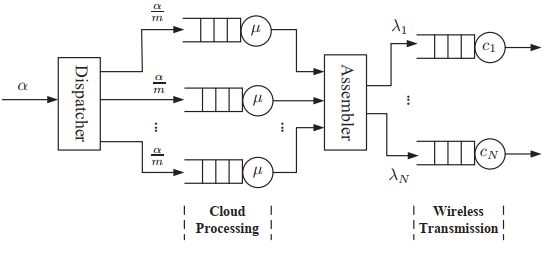
\includegraphics[scale = 0.7]{./fig/Delay}
  \caption{مدل پردازشی شبکه صف \cite{frdl}.}
  \label{fig:Delay}
\end{figure}
همانطور که در شکل \eqref{fig:Delay}، مشخص است، در این شبکه برای هر بخش تعدادی VNF قرار دارند که پردازش ها را انجام می‌دهند. در مسیر لینک پایین
بسته ها با نرخ $\alpha$ به صف های مختلف وارد شده و پس از پردازش با همدیگر ادغام شده و سپس بسته ی هر کاربر از طریق وایرلس منتقل میشوند.
در این پردازش ها، از روش M/M/1 استفاده شده‌است.
در این مدل مقالات اشاره ی مستقیم به برش شبکه نشده‌است ولی
در آنها ترکیبی از مفهوم برش RAN و Core به چشم می‌خورد.
\subsection{رفتن به سمت شبکه های دسترسی رادیویی باز}
در فوریه 2018 ، شبکه دسترسی رادیویی آزاد (O-RAN) با ادغام  xRAN و اتحاد C-RAN برای ایجاد سطح جدیدی از باز بودن در شبکه دسترسی رادیویی ایجاد شد که از نسل 5G و 6G پشتیبانی می‌کند.
هدف اصلی O-RAN افزایش عملکرد RAN از طریق عناصر شبکه مجازی و واسط های باز است که دارای هوش در RAN است.
صراحت و هوش دو ستون اصلی تلاشهای انجام شده توسط اتحاد O-RAN است که یک نیروی جهانی متشکل از بیش از 160 شرکت کننده از فروشندگان بزرگ ، شرکت های کوچک و متوسط ، اپراتورهای شبکه ، مبتدیان و مؤسسات دانشگاهی است
\cite{oranpaper}
.

در مقاله‌ی 
\cite{oranInt}
 مقدمه ای در مورد مفاهیم، اصول و الزامات \lr{Open RAN} که توسط اتحاد O-RAN مشخص شده، بیان شده‌است.
 در این مقاله،
 به منظور نشان دادن نقش هوش در O-RAN، طرح مدیریت منابع رادیویی هوشمندی را برای رسیدگی به ازدحام ترافیک و نشان دادن اثربخشی آن در یک مجموعه داده در دنیای واقعی پیشنهاد شده‌است.
 یک معماری سطح بالا از این سناریوی استقرار که سازگار با الزامات O-RAN است نیز مورد بحث قرار گرفته است. مقاله با چالشهای کلیدی فنی و مشکلات باز برای تحقیقات و توسعه آینده به پایان میرسد.
 
در مقاله‌ی
\cite{c2o}
تعاریف عمومی، ویژگی های اساسی و روند تحقیقاتی فعلی در شبکه های دسترسی رادیویی ابری و مشتقات آن، شبکه های دسترسی رادیویی مجازی و شبکه های دسترسی رادیویی باز ارائه شده‌است.
علاوه بر این، نتایج عملی و آموزه های آموخته شده در مورد محدودیت ها و مسائل پیش بینی نشده مجازی سازی شبکه های دسترسی رادیویی را ارائه داده شده‌است.

در مقاله‌ی 
\cite{sree2019open, kawahara2019ran}
 ساختار و مدیریت منابع رادیویی (RRM) هوشمند 
 و همچنین نقش مدیریت لینک رادیویی (RLM) در بهینه سازی انرژی در RRM
در نظر گرفته شده‌است.
ساختار RLM در 
زیرساخت O-RAN مورد بررسی قرار گرفته است.
علاوه بر این، دیدگاه
O-RAN
 و معماری آن مورد توجه قرار گرفته است.
\subsection{قرار دادن VNF ها}
NFV
 الگویي است که عملکردهای شبکه سنتی را مجازی می‌کند و آنها را در سخت افزارهای عمومی و ابرها در مقابل سخت افزارهای تعیین شده، قرار می‌دهد.
 در واقع NFV بخش نرم افزار را از سخت افزار جدا می‌نماید.
 بنابراین یک سرویس داده شده میتواند به مجموعه ای از توابع شبکه مجازی (VNF) تجزیه شود ، سپس میتوان آن را در نرم افزارهایی که روی یک یا چند سرور استاندارد فیزیکی صنعت اجرا میشوند ، پیاده سازی کرد.
 
اپراتورهای شبکه تلفن همراه عهده دار تصمیم گیری مدیریت زیرساخت است.
این وظیفه بخشی از تنظیمات شبکه است و شامل تصمیم گیری در مورد قرار دادن VNF های مورد نیاز در سراسر زیرساخت و اختصاص پردازنده، حافظه و منابع ذخیره سازی به VNF ها و مسیریابی داده ها از طریق گره های شبکه
می‌باشد.

به لطف برش شبکه، شبکه های 5G از انواع خدمات به روشی انعطاف پذیر و سریع پشتیبانی میکنند. در این زمینه ، ما به دنبال تصمیم گیری بهینه و با کیفیت بالا در مورد قرار دادن VNF در میان میزبانهای فیزیکی برای تحقق بخشیدن به خدمات هستیم.

در مقالات
\cite{wang2016online,jia2018online,luo2020online}
هدف یافتن تعداد بهینه ی VNF ها در یک زنجیره ی سرویس و قرار گیری VNF های مورد نظر بر روی سرور در هر بازه ی زمانی می‌باشد تا بتوان میزان هزینه را در سیستم به حداقل رساند.
در این مقالات هدف کمینه کردن انرژی های مصرفی در هر بازه ی زمانی می‌باشد که شامل هزینه ی انرژی مصرفی هر VNF مستقر بر روی سرور در حال کار و هزینه ی استقرار VNF های جدید در هر لحظه ی زمانی می‌باشد.
همچنین مجموع منابع مصرفی VNF های مستقر بر روی هر سرور در هر لحظه میبایست از منابع آن سرور کمتر باشد تا مساله عملی شود.
با استفاده از الگوریتم آنلاین این مساله حل شده‌است.‌
در مقاله‌ی 
\cite{jia2018online,luo2020online}
نرخ جریان هر VNF و سرور نیز در نظر گرفته شده‌است و دیتا سنترها و VNF ها به صورت گرافی شبیه سازی شده‌اند.
در مقاله‌ی
\cite{luo2020online}
الگوریتم روند کردن استفاده کرده که نتیجه ی خوبی را در مقابل مساله ی آفلاین دارد.

در مقاله‌ی
\cite{cziva2018dynamic}
مساله ی قرار دادن VNF ها در لبه مورد بررسی قرار می‌گیرد که در اینجا تخصیص VNF ها در یک سیستم با زیرساخت لبه مورد توجه قرار گرفته است و هدف کمینه کردن تاخیر انتها به انتها از هر کاربر به VNF مورد نظر آن می‌باشد و از روش دینامیکی و پویا برای حل مساله استفاده شده‌است. 

در مقاله‌ی
\cite{pei2019optimal}
مساله ی قرار دادن VNF در شبکه های فعال SDN/NFV مطالعه شده‌است، که به طور طبیعی به عنوان یک مساله ی برنامه نویسی باینری (BIP) فرموله شده‌است. 
در این مساله قرارگیری VNF زنجیر عملکرد سرویس مورد بررسی قرار گرفته شده‌است. 
با استفاده از روش یادگیری تقویت عمیق، الگوریتم قرارگیری VNF مبتنی بر شبکه DDQN \LTRfootnote{Double Deep Q-learning} پیشنهاد می‌کنیم.

در مقاله‌ی
\cite{ren2020joint}
 مسئله ی بهینه سازی مشترک قرار دادن VNF ها و زمانبندی جریان مطالعه شده‌است.
 این مساله از نوع برنامه نویسی عدد صحیح می‌باشد.
 برای حالت تک جریان، مساله به سادگی قابل حل است اما برای جندین جریان مساله
 NP-hard
 خواهد بود و با استفاده از روش relax کردن لاگرانژ
 قابل حل می‌باشد.
\section{روش های حل}
در این بخش مروری بر حل مسائل توسط مقالات می‌نماییم. 
ابتدا به دو مسئله ی معروف NP-Hard
اشاره می‌کنیم سپس به حل مسائل با استفاده از روش یادگیری تقویتی می‌پردازیم.
\subsection{مسائل Np-Hard}
در اینجا به دو مسئله‌ی کوله پشتی و بسته بندی جعبه می‌پردازیم. این دو مسئله NP-Hard هستند.
مسئله‌ی NP-hard را نمی‌توان در زمان چند جمله‌ای حل کرد در نتیجه از روشهای ابتکاری برای رسیدن به جواب نزدیکه بهینه استفاده می‌شود.
\subsubsection{ مسئله‌ی کوله‌پشتی }
یکی از مسائل پیش رو، مسئله ی کوله پشتی \LTRfootnote{knapsack}
می‌باشد.
این مسئله، از جنس NP-hard
می‌باشد که در این مسئله میخواهیم تعدادی شی با وزنهای مختلف را در تعدادی جایگاه با ظرفیت مشخص قرار دهیم.
هدف در این مسئله قرارگیری بیشترین تعداد اشیاء در این جایگاه ها می‌باشد.
حل این مسئله با استفاده از روش های مختلف صورت می‌گیرد.

در مقاله‌ی \cite{lee2018dynamic}
همانطور که قبل تر اشاره شد، مسئله ی پذیرش کاربر و ارتباط کاربر از جنس کوله پشتی
 می‌باشد که به ترتیب با استفاده از الگوریتم دینامیکی و الگوریتم حریص تعریف شده در مقاله
 حل می‌گردد.

در مقاله‌ی
\cite{sciancalepore2017mobile}
یک راه حل جامع شامل برش شبکه، پیش بینی ترافیک، کنترل پذیرش و برنامه ریزی برای یک سیستم شامل برش شبکه 5G ارائه شده‌است.
راه حل کنترل پذیرش به یک مسئله کوله پشتی هندسی (دو بعدی) ترسیم شده و دو الگوریتم کم پیچیدگی به ترتیب برای درخواست های برش شبکه منظم و نامنظم طراحی شده‌اند. 
\subsubsection{مسئله‌ی بسته‌بندی جعبه}
 در این مسئله هدف قرار دادن تعدادی شیء در تعدادی جعبه با ظرفیت مشخص می‌باشد.
در مسئله ی بسته بندی جعبه \LTRfootnote{bin packing}
هدف کمینه کردن تعداد جعبه های ورودی با فرض اینکه همه ی اشیا در آن جا شوند.

در مقاله‌ی
\citep{wang2017joint}
مسئله ی تخصیص منابع و بدست آوردن انرژی بهینه در ساختار
H-CRAN
می‌باشد.
در این مقاله هدف تخصیص همزمان منابع ایستگاه رادیویی RRH و باند پایه BBU می‌باشد.
این مسئله به دو بخش مجزا برای تخصیص منابع هر بخش شکسته می‌شود.
بخش دوم که مربوط به زمان بندی و برنامه ریزی BBU می‌باشد به فرم یک مسئله ی باینری بسته بندی جعبه نوشته می‌شود.
برای حل این الگوریتم از روش های مختلفی از جمله
Next-Fit(NF)
First-Fit(FF)،
First-Fit-Decreasing(FFD)،
و
‌Best-Fit-Decreasing(BFD)
می‌باشد که الگوریتم به کار رفته در مسئله از نوع روش
BFD 
 است که جواب بهتری در مقایسه با روشهای دیگر دارد.  
 
در مقاله‌ی
\cite{de2020optimal}
به صورت همزمان قرار دادن VNF ها و تخصیص منابع محاسباتی مورد هدف قرار داده شده‌است.
این مسئله به صورت
برنامه نویسی خطی 
mixed-integer
می‌شود که بعد از تغییرات به صورت برنامه نویسی خطی عدد صحیح میتوان نوشت که به فرم مسئله ی بسته بندی جعبه خواهد بود که با استفاده از الگوریتم مشابه
BFD حل می‌گردد.
\subsection{روشهای یادگیری تقویتی}
در این بخش تمرکز ما بر‌روی مقالاتی است که از روش یادگیری عمیق در حل مسئله استفاده می‌کند. 
یادگیری تقویتی
 \LTRfootnote{Reinforcement Learning}
 در حال حاضر یکی از موضوعات داغ پژوهشی محسوب می‌شود و محبوبیت آن روز به روز در حال افزایش است.
یادگیری تقویتی گونه‌ای از روش‌های یادگیری ماشین است که یک عامل(agent) را قادر به یادگیری در محیطی تعاملی با استفاده از آزمون و خطاها و استفاده از بازخوردهای اعمال و تجربیات خود می‌سازد. اگرچه هم یادگیری نظارت شده و هم یادگیری تقویتی از نگاشت بین ورودی و خروجی استفاده می‌کنند، اما در یادگیری تقویتی که در آن بازخوردهای فراهم شده برای عامل، مجموعه صحیحی از اعمال، جهت انجام دادن یک وظیفه هستند، بر خلاف یادگیری نظارت شده از پاداش‌ها و تنبیه‌ها به عنوان سیگنال‌هایی برای رفتار مثبت و منفی بهره برده می‌شود. 
  در یادگیری تقویتی هدف پیدا کردن مدل داده مناسبی است که پاداش کل را برای عامل، بیشینه می‌کند. تصویر زیر ایده اساسی و عناصر درگیر در یک مدل یادگیری تقویتی را نشان می‌دهد.
\begin{figure}
  \centering
    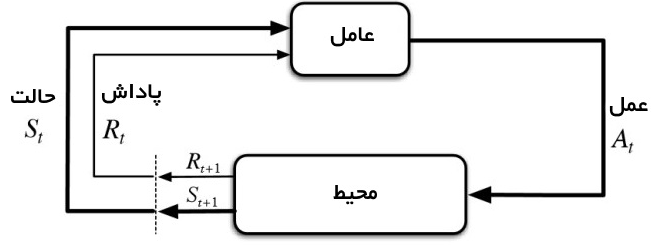
\includegraphics[scale=0.7]{./fig/rl}
  \caption{یادگیری تقویتی}
  \label{fig:rl}
\end{figure}
برخی از اصطلاحاتی که عناصر یک مساله یادگیری تقویتی را تشریح می‌کنند در ادامه بیان شده‌است.
\begin{itemize}
\item محیط (Environment):
 جهان فیزیکی که عامل در آن عمل می‌کند.
\item حالت (State):
 موقعیت کنونی عامل
\item پاداش (Reward):
 بازخورد از محیط
\item  سیاست (Policy):
 روشی برای نگاشت حالت عامل به عمل
\item  ارزش (Value):
 پاداش آینده که یک عامل با اقدام به یک عمل در یک حالت خاص به آن دست می‌یابد.
\end{itemize}
یادگیری تقویتی عمیق
DRL \LTRfootnote{Deep Reinforcement Learning}،
 از شبکه‌های عصبی عمیق برای حل مسائل یادگیری تقویتی استفاده می‌کند، از این رو در نام آن از کلمه عمیق استفاده شده‌است. با در نظر گرفتن Q-Learning که یادگیری تقویتی کلاسیک محسوب می‌شود و Deep-Q-Learning می‌توان تفاوت آن‌ها با یکدیگر را دید. در رویکرد اول، از الگوریتم‌های سنتی برای ساخت جدول Q استفاده می‌شود تا به عامل در یافتن اقدامی که باید در هر حالت انجام شود کمک کند. در دومین رویکرد، از شبکه عصبی (برای تخمین پاداش بر مبنای حالت: مقدار q) استفاده می‌شود.

در مقاله‌ی
 \cite{gan1, gan2}
سناریویی در نظر گرفته شده‌است که شامل چندین برش در یک شبکه دسترسی رادیویی با ایستگاههای پایه است که از منابع فیزیکی مشترک (به عنوان مثال، پهنای باند) استفاده میکنند. 
با استفاده از یادگیری تقویت عمیق (DRL) با در نظر گرفتن تقاضای مختلف خدمات به عنوان وضعیت محیط و منابع اختصاص یافته به عنوان عمل محیط، این مشکل حل می‌شود.
برای کاهش نویز و رسیدن به سطح انتظار خدمات، از روش GAN در بخش عمیق الگوریتم استفاده شده‌است که منجر به حداقل رساندن اختلاف بین توزیع مقدار-عمل تخمین زده شده و توزیع ارزش عمل هدف
می‌شود.
برای یافتن سیاست بهینه ی تخصیص منابع از روش
DDQN \LTRfootnote{Double Deep Q-Network}
 استفاده می‌شود.
\begin{figure}
  \centering
    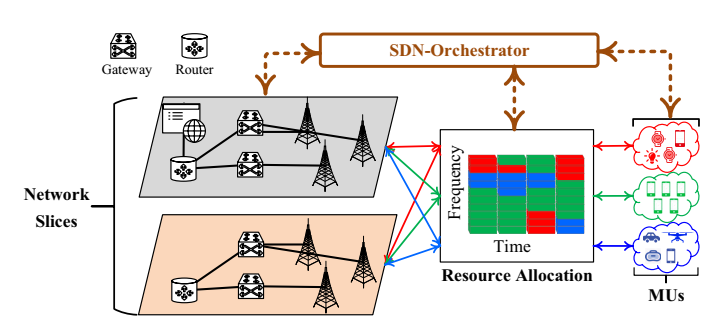
\includegraphics[scale=0.7]{./fig/gan}
  \caption{سناریوی ارسال لینک بالا و پایین در برشهای شبکه }
  \label{fig:gan}
\end{figure} 
 
در مقاله‌ی
\cite{li2020end} 
الگوریتم تخصیص منابع برش شبکه انتها به انتها مبتنی بر 
DQN \LTRfootnote{deep Q-Network}
 پیشنهاد شده‌است که برای سناریوهای چند برش و چند سرویس مناسب است.
 در این سیستم دو مدل سرویس ارائه شده‌است که اولی بر مبنای نیاز به رسیدن به نرخ خاص و دومی نیازمند داشتن تاخیر کم می‌باشد.
هدف در این سیستم رسیدن به بیشینه نرخ دسترسی است.
برای رسیدن به هدف مورد نظر برشها به دو بخش دسترسی و اصلی تقسیم شده‌اند.
 در اینجا الگوریتم به طور مشترک برشهای شبکه دسترسی رادیویی و برشهای شبکه اصلی را در نظر می‌گیرد تا منابع را به صورت دینامیکی طوری اختصاص دهد که 
 حداکثر میزان کاربران به شبکه دسترسی داشته و به بیشینه نرخ برسد.
 این سیستم به صورت برنامه ی
 mixed-integer
 نوشته می‌شود
و مسئله به صورت دو مسئله ی کوله پشتی و اتصال لینک ها بیان می‌شود
  و با استفاده از روش
 DQN
 حل می‌گردد.
 